
%%%%%%%%%%%% FOLHA DE APROVACAO %%%%%%%%%%%%%%%%%%%%%%

% INSERINDO FOLHA DE ASSINATURAS PREENCHIDA
\begin{center}
 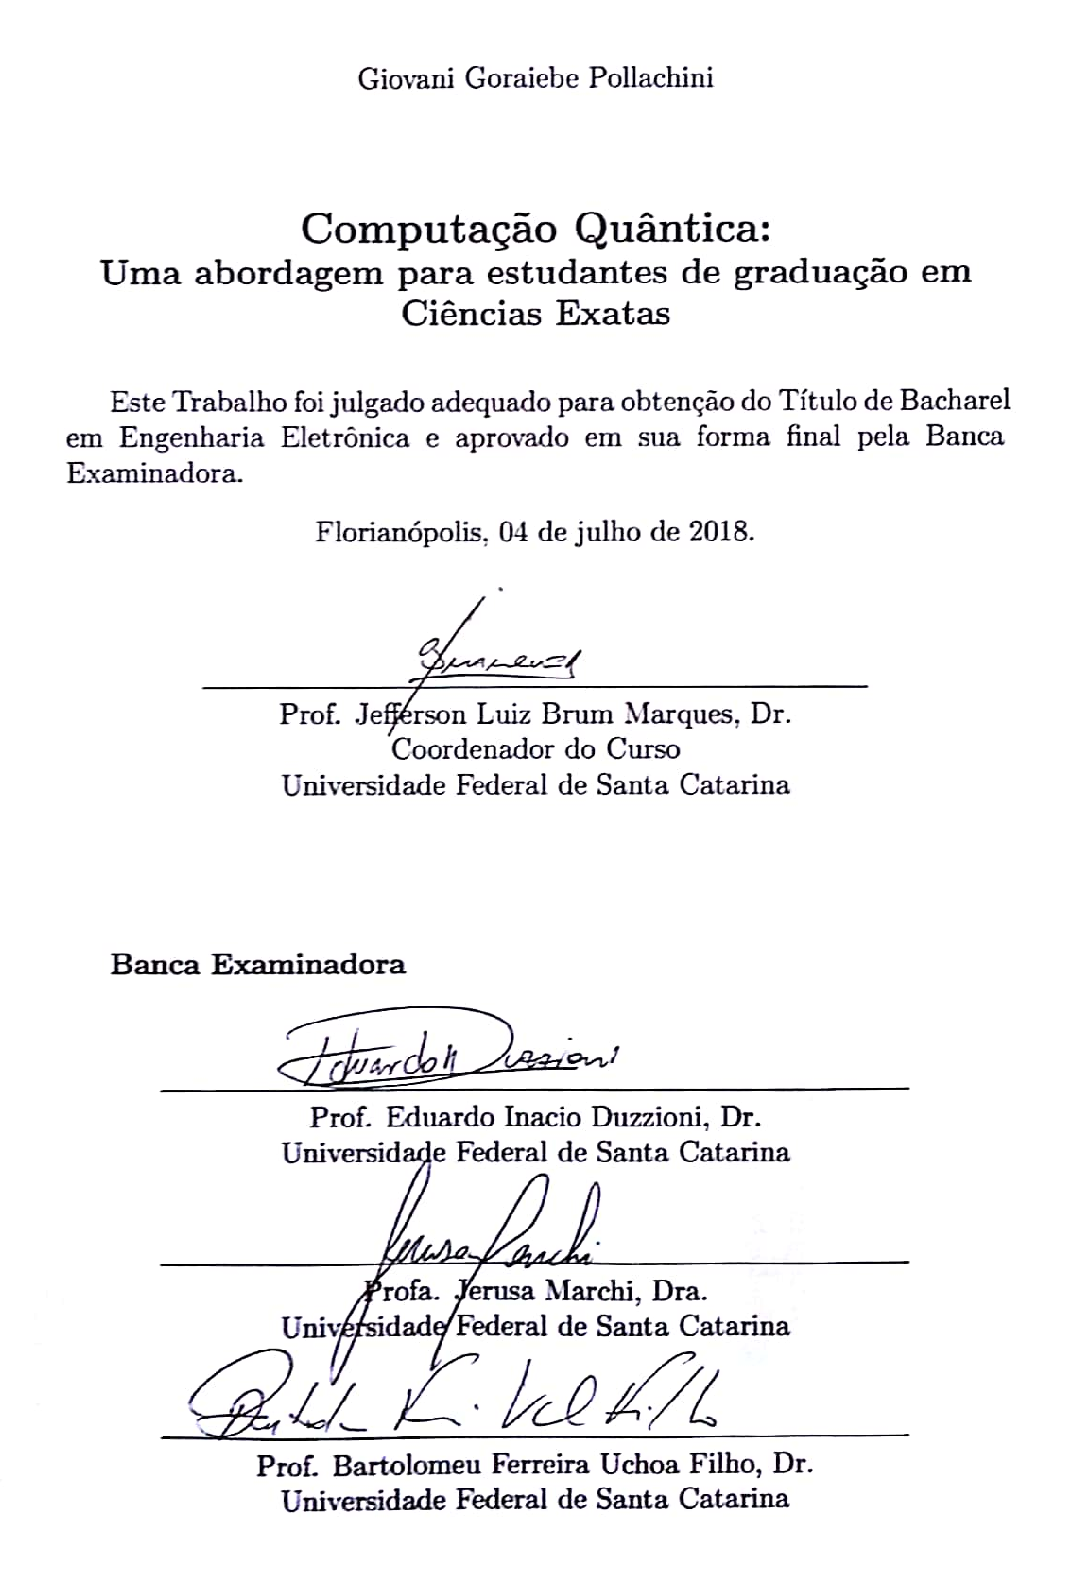
\includegraphics[scale=0.65]{folha_assinatura/folha_assinatura_preenchida}
\end{center}

\begin{comment}
\begin{center}
 { Giovani Goraiebe Pollachini
}\end{center}

\vspace*{0.5 cm}

\begin{center}
 \Large{\bf Computa��o Qu�ntica:} \\
 \large{\bf \nohyphens{Uma abordagem para estudantes de gradua��o em Ci�ncias Exatas}}
\end{center}

\vspace{0.25 cm}
\nohyphens{Este Trabalho foi julgado adequado para obten��o do T�tulo de Bacharel em Engenharia Eletr�nica e aprovado em sua forma final pela Banca Examinadora.}
\begin{center}
Florian�polis, 04 de julho de 2018.
\end{center}

\vspace{1cm}

\begin{center}
\begin{minipage}{8cm}
\begin{center}
\hrulefill\\
Prof. Jefferson Luiz Brum Marques, Dr.
\\
Coordenador do Curso
\\
Universidade Federal de Santa Catarina
\end{center}
\end{minipage}
\end{center}

\vspace*{1.5 cm}

{\bf Banca Examinadora}

\vspace{1 cm}

\begin{center}
\begin{minipage}{9cm}
\begin{center}
\hrulefill\\
{ Prof. Eduardo Inacio Duzzioni, Dr.\\ Universidade Federal de Santa Catarina}\\
\vspace*{0.8 cm}
\hrulefill\\
{ Profa. Jerusa Marchi, Dra. \\ Universidade Federal de Santa Catarina}\\
\vspace*{0.8 cm}
\hrulefill\\
{ Prof. Bartolomeu Ferreira Uchoa Filho, Dr. \\ Universidade Federal de Santa Catarina}\\
\end{center}
\end{minipage}
\end{center}

\end{comment}

\newpage
\textcolor{white}{\ }

\newpage